\section{Experimentación}

\subsection{Descripción de la Experimentación}

En esta sección se cubre la parte técnica del proyecto. El objetivo principal consiste en la implementación de los diferentes métodos y técnicas que se han tratado a lo largo del documento. Adicionalmente, se busca presentar los resultados obtenidos en los distintos casos prácticos. Por último, se incluye un análisis e interpretación de los resultados haciendo especial énfasis en la curva-A.

\bigbreak

La experimentación que se propone esta compuesta por seis casos prácticos, cada caso práctico tiene asociado un fichero de datos diferente. Los ficheros que se utilizan forman parte de un repositorio de datos creado especialmente para su aplicación en la evaluación de modelos predictivos \cite{Feltes2019}. La temática del repositorio esta relacionada con el estudio de diferentes tipos de cáncer, el uso de este repositorio supone una excelente elección, ya que cubre un amplio número de casuísticas. En la página web SBCB \cite{SBCB} se puede encontrar una recopilación de los distintos ficheros de datos que incluye el repositorio. 

\bigbreak

Los ficheros de datos se han seleccionado para su aplicación tanto a modelos de clasificación binaria como a modelos de clasificación multi etiqueta. Los ficheros que se han seleccionado para modelos de clasificación binaria son leukemia\_gse14317, gastric\_gse79973 y breast\_gse42568. Los ficheros que se han seleccionado para modelos de clasificación multi etiqueta son colorectal\_gse21510, breast\_gse45827 y brain\_gse15824. El escenario de pruebas es común para todos los casos prácticos, en el escenario de pruebas que se define no se realiza ningún tipo de preprocesado al conjunto de datos de entrada. El predictor que se ha seleccionado es un predictor bayesiano, para mejorar el rendimiento del predictor se aplica una normalización al conjunto de datos. En la fase de validación se aplica validación cruzada con 10 iteraciones, el uso de este método está ampliamente extendido en proyectos de este tipo, ya que ofrece grandes resultados.

\bigbreak

La implementación se ha realizado utilizando la herramienta Knime. El flujo principal esta definido para la ejecución automática de una batería de ficheros (Anexo I). El usuario una vez finalizada la ejecución puede exportar los resultados en varios formatos, los resultados también se pueden visualizar en Knime a través del componente REPORT.

\clearpage

\subsection{Resultados de la Experimentación}

%%%%%%%%%%%%%%%%%%%%%%%%%%%%%%%%%%%%%%%%%%%%%%%%%%%%%%% RESULTADO
\subsubsection{Fichero brain\_gse15824.csv}

\begin{table}[htp]
    \small
    \centering
    \begin{tabularx}{\columnwidth}{Y Y}
        ACC       & AUAC    \\\hline
        $0.757$   & $0.764$ \\\hline
    \end{tabularx}
    \caption{Resultados globales para el fichero brain\_gse15824.csv.}
    \label{tab:10}
\end{table}

\begin{table}[htp]
    \small
    \centering
    \begin{tabularx}{\columnwidth}{l c c c c}
                &  Astrocytoma  & Glioblastoma & Oligodendrioglioma   & Glioblastoma-cell-line   \\\hline
        TPR     &  $0.500$      & $1.000$      & $0.286$              & $1.000$                  \\\hline
        TNR     &  $0.966$      & $0.720$      & $0.967$              & $1.000$                  \\\hline
        PPV     &  $0.800$      & $0.632$      & $0.667$              & $1.000$                  \\\hline
        NPV     &  $0.875$      & $1.000$      & $0.853$              & $1.000$                  \\\hline
        LR+     &  $14.500$     & $3.571$      & $8.571$              & -                        \\\hline
        LR-     &  $0.518$      & $0.000$      & $0.739$              & $0.000$                  \\\hline
        DOR     &  $28.000$     & -            & $11.600$             & -                        \\\hline
        YI      &  $0.466$      & $0.720$      & $0.252$              & $1.000$                  \\\hline
        MCC     &  $0.561$      & $0.674$      & $0.362$              & $1.000$                  \\\hline
        DP      &  $0.798$      & -            & $0.587$              & -                        \\\hline
        $F_{1}$ &  $0.615$      & $0.774$      & $0.400$              & $1.000$                  \\\hline
        MK      &  $0.675$      & $0.632$      & $0.520$              & $1.000$                  \\\hline
        BCR     &  $0.733$      & $0.860$      & $0.626$              & $1.000$                  \\\hline
        GM      &  $0.695$      & $0.849$      & $0.526$              & $1.000$                  \\\hline
        OP      &  $0.547$      & $0.648$      & $0.294$              & $1.000$                  \\\hline
        Jaccard &  $0.444$      & $0.632$      & $0.250$              & $1.000$                  \\\hline

    \end{tabularx}
    \caption{Resultados agrupados por clase para el fichero brain\_gse15824.csv.}
    \label{tab:11}
\end{table}

\bigbreak

\begin{figure}[htp]
    \centering
     \subfloat[Curva ROC]{
       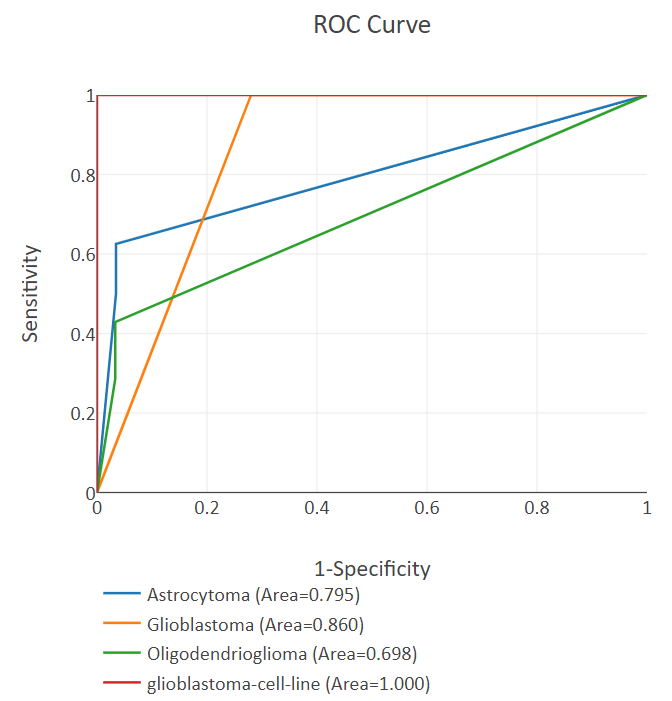
\includegraphics[width=0.4\textwidth]{brain_gse15824_ROC.PNG}}
     \subfloat[Curva A]{
       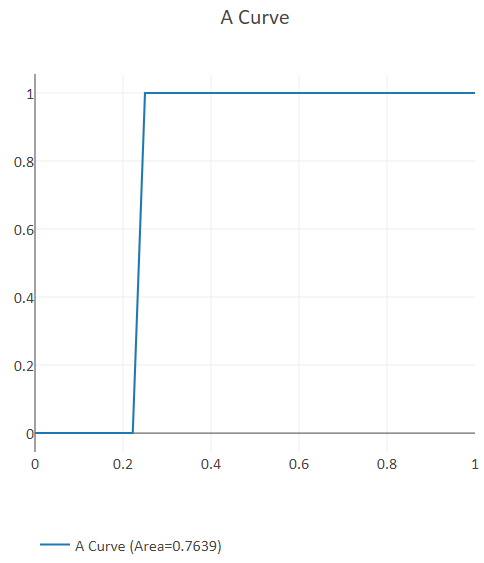
\includegraphics[width=0.4\textwidth]{brain_gse15824_A_CURVE.PNG}}
    \caption{Curvas obtenidas para el fichero brain\_gse15824.csv.}
    \label{fig:10}
\end{figure}

\bigbreak

El fichero de datos brain\_gse15824.csv presenta cuatro clases, los nombres de las clases son Astrocytoma, Glioblastoma, Oligodendrioglioma y Glioblastoma-cell-line. En esta sección se propone un análisis e interpretación de los resultados obtenidos al aplicar los métodos de evaluación vistos en secciones anteriores. El análisis e interpretación se realiza de forma independiente para las distintas clases.

\bigbreak

La exactitud presenta un $75.7$\% de probabilidad de acierto en la predicción. El área bajo la curva-A obtiene un resultado que muestra una notable capacidad predictiva, la diferencia entre el área bajo la curva-A y la exactitud es de 0,007 unidades. La curva ROC representa de forma gráfica el comportamiento de cada una de las clases, las etiquetas Astrocytoma y Oligodendrioglioma obtienen una representación similar, en ambos casos la curva muestra una capacidad discriminatoria aceptable. La clase Glioblastoma presenta una importante mejora con respecto a las clases Astrocytoma y Oligodendrioglioma, los resultados indican que el modelo obtiene una tasa de aciertos considerable para esta clase. Por último, la clase Glioblastoma-cell-line presenta un comportamiento perfecto. La curva-A ofrece también una representación del comportamiento del modelo, la representación establece que el modelo tiene una notable calidad predictiva.

\bigbreak

La clase Astrocytoma muestra una sensibilidad reducida, tan solo la mitad de los registros de está clase se predicen de forma correcta. La especificidad establece que el 96,6\% de los registros con una clase diferente a Astrocytoma no se predicen de clase Astrocytoma. La precisión indica que los registros que se predicen de clase Astrocytoma tienen una tasa de acierto del 80\%. La precisión inversa establece que el 87,5\% de los registros no son de clase Astrocytoma cuando se predicen de una clase distinta a Astrocytoma. La razón de verosimilitud positiva presenta un fuerte aumento en la probabilidad de acierto que tiene un registro que se predice de clase Astrocytoma, en concreto supone más de un 45\% de mejora (Tabla \ref{tab:2}). La razón de verosimilitud negativa muestra una leve reducción en la probabilidad de que un registro sea de clase Astrocytoma cuando se predice de otra clase, la reducción que presenta es de entorno al 15\% (Tabla \ref{tab:2}). El DOR ofrece un indicador conjunto de las razones de verosimilitud, en general el modelo presenta una buena capacidad discriminatoria para la clase Astrocytoma. El indice de Youden tiene un valor de $0.46$, un valor poximo a $0.5$ indica una capacidad discriminatoria aceptable para la clase Astrocytoma. El resultado para el coeficiente de correlación de Matthews es de $0.561$ puntos, un valor que indica una fuerte correlación entre clase y predicción (Tabla \ref{tab:3}). El poder discriminante de $0.798$ implica una capacidad discriminatoria postiva para la clase Astrocytoma. El valor de la medida-F implica una tasa aceptable de acierto para instancias en las que la clase o la predicción es Astrocytoma, en este caso la baja sensibilidad obtenida penaliza el resultado obtenido. El \textit{markedness} es un indicador que agrupa los métodos que miden la exactitud en la predicción, un resultado de $0.675$ implica una notable tasa de acierto. La media geométrica y la exactitud balanceada ofrecen un indicador de la tasa de aciertos conjunta para instancias de clase Astrocytoma e instancias que no son de clase Astrocytoma, en ambos casos el indicador es notablemente alto. El resultado para la precisión de optimización es de $0.547$ puntos, un valor bajo que se ha visto afectado por la gran diferencia que existe entre sensibilidad y especificidad. El resultado que se obtiene al aplicar Jaccard es de $0.444$ puntos, esto indica un grado de similitud bajo entre clase y predicción.

\bigbreak

La sensibilidad para la clase Glioblastoma es de una unidad, esto implica que todas las instancias de esta clase se clasifican de forma correcta. El indicador de especificidad indica una notable tasa de acierto a la hora de determinar que instancias no pertenecen a la clase Glioblastoma. La precisión de $0.63$ puntos implica una buena tasa de acierto sobre las instancias que se predicen de clase Glioblastoma. La precisión inversa obtiene un resultado de una unidad, la predicción es correcta para todas las instancias que se predicen de una clase diferente a Glioblastoma. La razón de verosimilitud positiva indica un leve aumento (Tabla \ref{tab:2}) en la probabilidad de que una instancia pertenezca a la clase Glioblastoma cuando se predice de esta clase. El indice de Youden indica una capacidad discriminatoria notable para la clase Glioblastoma. El resultado obtenido por el coeficiente de correlación de Matthews es de $0.674$, este valor implica una alta correlación (Tabla \ref{tab:3}) entre la predicción y la clase Glioblastoma. La medida-F indica una tasa notable de acierto en la predicción de la clase. La media geométrica y la exactitud balanceada ofrecen indicadores que reflejan una tasa de aciertos notable, ambos métodos agrupan sensibilidad y especificidad. La precisión de optimización indica una buena tasa de acierto para la clase Glioblastoma. El método de Jaccard indica un grado de similitud medio entre la predicción y la clase Glioblastoma.

\bigbreak

La clase Oligodendrioglioma presenta una sensibilidad de $0.286$, tan solo el $28.6$\% de instancias de esta clase se predicen de forma correcta. La especificidad es de $0.967$, este valor indica un excelente comportamiento del modelo sobre instancias con una clase diferente a Oligodendrioglioma. El resultado obtenido para la precisión es aceptable, la tasa acierto sobre las instancias que se predicen positivas supera el $66$\%. La precisión inversa presenta un resultado notablemente alto, la predicción es correcta para el $85.3$\% de instancias que se predicen de una clase distinta a Oligodendrioglioma. La razón de verosimilitud positiva indica una aumento en la probabilidad de que una instancia sea Oligodendrioglioma cuando se predice de esta clase, el aumento es de entre el 30\% y el 40\% de que la clase. La razón de verosimilitud negativa obtiene un valor muy cercano a la unidad, la disminución de la probabilidad de que la clase sea Oligodendrioglioma cuando la instancias se predice de otra clase es muy leve. EL indice de Youden y el DOR indican una capacidad discriminatoria moderada entre la clase Oligodendrioglioma y el resto. El coeficiente de correlación de Matthews presenta una correlación entre clase y predicción moderada para la clase Oligodendrioglioma. EL resultado de la medida-F indica tasa reducida de acierto para la clase Oligodendrioglioma, la baja sensibilidad penaliza el resultado. El \textit{markedness} ofrece un indicador del acierto en la predicción de la clase Oligodendrioglioma frente al resto, el resultado que se obtiene indica un acierto en la predicción moderado. La media geométrica y la exactitud balanceada presentan una tasa de aciertos reducida. La precisión de optimización indica una muy reducida tasa de acierto para la clase Oligodendrioglioma, la diferencia entre sensibilidad y especificidad afecta notablemente al resultado final. El método de Jaccard obtiene un resultado bajo, esto implica un grado de similitud reducido entre la clase Oligodendrioglioma y la predicción.

\bigbreak

La clase Glioblastoma-cell-line muestra un comportamiento ideal, el modelo es capaz de discriminar entre esta clase y el resto de forma perfecta.

\bigbreak

Los resultados obtenidos para el fichero brain\_gse15824.csv han sido positivos, en general las tasas de acierto han sido notables. Los métodos que se aplicado ayudan a reconocer algunos puntos de mejora, en este caso, la clase Oligodendrioglioma es la que obtiene peores indicadores, el modelo puede mejorarse ajustando la predicción sobre esta clase.

\clearpage

%%%%%%%%%%%%%%%%%%%%%%%%%%%%%%%%%%%%%%%%%%%%%%%%%%%%%%% RESULTADO

\subsubsection{Fichero breast\_gse45827.csv}

\begin{table}[htp]
    \small
    \centering
    \begin{tabularx}{\columnwidth}{Y Y}
        ACC       & AUAC    \\\hline
        $0.914$   & $0.917$ \\\hline
    \end{tabularx}
    \caption{Resultados globales para el fichero breast\_gse45827.csv.}
    \label{tab:12}
\end{table}

\begin{table}[htp]
    \small
    \centering
    \begin{tabularx}{\columnwidth}{l Y Y Y Y Y Y}
                &  Her          & Basal     & Cell\_line & Luminal\_a & Luminal\_b & Normal    \\\hline
        TPR     &  $0.900$      & $0.927$   & $1.000$    & $0.862$    & $0.933$    & $0.857$   \\\hline
        TNR     &  $0.967$      & $0.982$   & $1.000$    & $0.984$    & $0.959$    & $1.000$   \\\hline
        PPV     &  $0.871$      & $0.950$   & $1.000$    & $0.926$    & $0.848$    & $1.000$   \\\hline
        NPV     &  $0.975$      & $0.973$   & $1.000$    & $0.968$    & $0.983$    & $0.993$   \\\hline
        LR+     &  $27.225$     & $50.976$  & -          & $52.586$   & $22.587$   & -         \\\hline
        LR-     &  $0.103$      & $0.075$   & $0.000$    & $0.140$    & $0.070$    & $0.143$   \\\hline
        DOR     &  $263.250$    & $684.000$ & -          & $375.000$  & $324.800$  & -         \\\hline
        YI      &  $0.867$      & $0.909$   & $1.000$    & $0.846$    & $0.892$    & $0.857$   \\\hline
        MCC     &  $0.856$      & $0.916$   & $1.000$    & $0.869$    & $0.861$    & $0.923$   \\\hline
        DP      &  $1.334$      & $1.563$   & -          & $1.419$    & $1.385$    & -         \\\hline
        $F_{1}$ &  $0.885$      & $0.938$   & $1.000$    & $0.893$    & $0.889$    & $0.923$   \\\hline
        MK      &  $0.846$      & $0.923$   & $1.000$    & $0.894$    & $0.832$    & $0.993$   \\\hline
        BCR     &  $0.933$      & $0.954$   & $1.000$    & $0.923$    & $0.946$    & $0.929$   \\\hline
        GM      &  $0.933$      & $0.954$   & $1.000$    & $0.921$    & $0.946$    & $0.926$   \\\hline
        OP      &  $0.918$      & $0.938$   & $1.000$    & $0.894$    & $0.940$    & $0.916$   \\\hline
        Jaccard &  $0.794$      & $0.884$   & $1.000$    & $0.806$    & $0.800$    & $0.857$   \\\hline
    \end{tabularx}
    \caption{Resultados agrupados por clase para el fichero breast\_gse45827.csv.}
    \label{tab:13}
\end{table}

\bigbreak

\begin{figure}[htp]
    \centering
     \subfloat[Curva ROC]{
       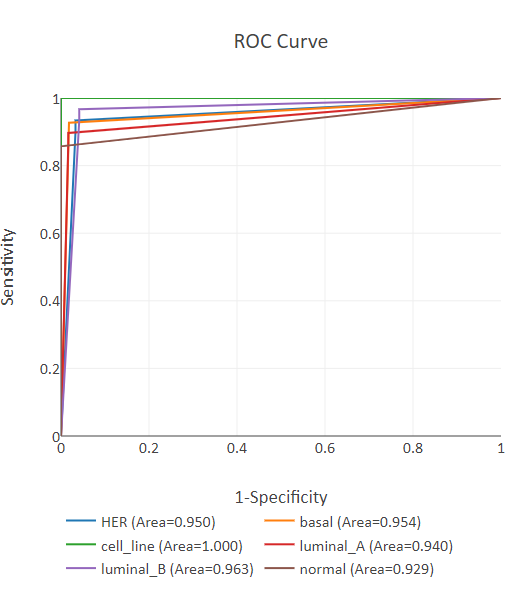
\includegraphics[width=0.4\textwidth]{breast_gse45827_ROC.PNG}}
     \subfloat[Curva A]{
       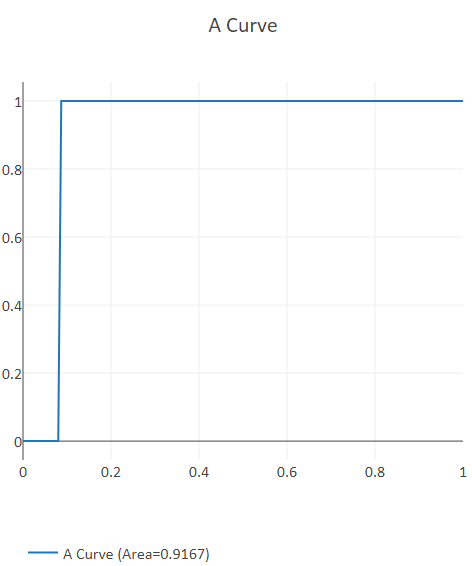
\includegraphics[width=0.4\textwidth]{breast_gse45827_A_CURVE.PNG}}
    \caption{Curvas obtenidas para el fichero breast\_gse45827.csv.}
    \label{fig:11}
\end{figure}

\bigbreak

El fichero de datos breast\_gse45827.csv presenta un total de seis etiquetas para la clase, los nombres de las etiquetas son Her, Basal, Cell\_line, Luminal\_a, Luminal\_b y Normal. En esta sección se propone un análisis e interpretación de los resultados obtenidos al aplicar los métodos de evaluación vistos en secciones anteriores. El análisis e interpretación se realiza de forma independiente para las diferentes clases.

\bigbreak

La exactitud presenta una excelente tasa de aciertos, la predicción es correcta para el 91,4\% de las instancias. La exactitud y el área bajo la curva-A obtienen un resultado similar, la diferencia entre ambos métodos supone un aumento de $0.003$ puntos del área bajo la curva-A sobre la exactitud. La curva ROC muestra una capacidad predictiva importante para todas las clases, las diferentes curvas muestran un grado de similitud notable entre sí. La curva-A ofrece una representación gráfica que muestra una excelente capacidad predictiva.

\bigbreak

La clase Her ofrece una sensibilidad considerable, la predicción sobre las instancias de esta clase se realiza con un 90\% de probabilidad de acierto. La especificidad obtiene un indicador sobresaliente, el 96,7\% de las instancias no se clasifican de clase Her cuando la clase real no es Her. La precisión establece que la predicción es correcta para el 87,1\% de las instancias que se predicen de clase Her. La precisión inversa indica que no se clasifican de clase Her el 97,5\% de las instancias con una predicción diferente a esta clase. La razón de verosimilitud positiva establece un fuerte aumento de la probabilidad de que se clasifique correctamente un registro que se predice de clase Her. La razón de verosimilitud negativa indica una importante reducción en la probabilidad de que un registro pertenezca a la clase Her cuando se clasifica de una clase diferente, la reducción de la probabilidad es de aproximadamente del 45\% (Tabla \ref{tab:2}). El DOR agrupa las razones de verosimilitud positiva y negativa, en general ofrece un gran indicador de la capacidad discriminante del modelo. El índice de Youden combina las medidas de sensibilidad y especificidad, el resultado muestra que el modelo discrimina de forma muy precisa entre la clase Her y el resto. El coeficiente de correlación de Matthews establece una fuerte correlación entre la clase Her y la predicción. El poder discriminante presenta un resultado que indica una capacidad discriminante aceptable entre la clase Her y el resto. La medida-F establece una buena capacidad predictiva para los registros en los que la clase o la predicción es Her. El \textit{markedness} combina los métodos de precisión y precisión inversa, el resultado representa una excelente capacidad discrimínate entre la clase Her y el resto. La media geométrica y la precisión balanceada ofrecen la media entre los indicadores de sensibilidad y especificidad, en ambos métodos el resultado presenta una tasa de acierto conjunta muy considerable. La precisión de optimización presenta la exactitud del modelo penalizando grandes diferencias entre sensibilidad y especificidad, el resultado ofrece un indicador notable. El método Jaccard indica un grado de similitud notable entre la clase Her y la predicción.

\bigbreak

La clase Basal presenta una sensibilidad excelente, el 90,2\% de los registros de esta clase se clasifican correctamente. La especificidad presenta un 98,2\% de probabilidad de acierto para los registros con una clase diferente a Basal. La precisión y la precisión inversa muestran resultados extraordinarios tanto para los registros que se predicen de clase Basal como para los que se predicen de otra clase. La razón de verosimilitud positiva indica un importante aumento en la probabilidad de que la predicción sea correcta para los registros  que se predicen de clase Basal. La razón de verosimilitud negativa establece una disminución en la probabilidad de que los registros que se predicen de una clase diferente a Basal se clasifiquen de clase Basal. El DOR es un método que combina las razones de verosimilitud, el resultado ofrece un indicador muy elevado de la capacidad discriminatoria entre la clase Basal y el resto. El índice de Youden presenta un excelente resultado de la capacidad discriminatoria que tiene el modelo. El coeficiente de correlación de Matthews indica una fuerte correlación entre la clase Basal y la predicción. La medida-F establece un indicador que agrupa los métodos de sensibilidad y precisión, el modelo presenta una gran capacidad predicativa sobre la clase Basal. El \textit{markedness} obtiene un resultado que indica una gran capacidad discriminatoria entre la clase Basal y el resto. La media geométrica y la exactitud balanceada presentan una tasa de acierto importante tanto para los registros de clase Basal como para los registro del resto de clases. La precisión de optimización obtiene un excelente indicador de la exactitud que presenta el modelo para la clase Basal, la penalización por la diferencia entre las medidas de sensibilidad y especificidad no tiene un gran impacto en el resultado final. El método de Jaccard establece un grado de similitud notable entre la clase Basal y la predicción.

\bigbreak

La clase Cell\_line presenta un comportamiento excelente, el modelo es capaz de discriminar entre esta clase y el resto de forma perfecta.

\bigbreak

La clase Luminal\_a presenta una sensibilidad notable, el 86,2\% de los registros de esta clase se predicen de forma correcta. La especificidad indica una excelente tasa de aciertos para los registros que pertenecen a una clase diferente a Luminal\_a. La precisión y precisión inversa establecen una extraordinaria tasa de acierto tanto para registros que se predicen de clase Luminal\_a como para registros que se predicen de otra clase diferente a Luminal\_a. La razón de verosimilitud positiva indica un fuerte aumento en la probabilidad de acierto para un registro que se predice de clase Luminal\_a. La razón de verosimilitud negativa ofrece un resultado que implica una reducción de la probabilidad de que los registros sean de clase Luminal\_a cuando se predicen de otra clase. EL indice de Youden indica una notable capacidad discriminatoria entre la clase Luminal\_a y el resto. El coeficiente de correlación de Matthews establece una fuerte correlación entre la clase Luminal\_a y la predicción. El poder discriminante indica que el modelo presenta una capacidad discriminatoria aceptable. La medida-F presenta un resultado excelente, la tasa de acierto es extraordinaria tanto para los registros de clase Luminal\_a como para los registros que se predicen de clase Luminal\_a. El \textit{markedness} establece una tasa de aciertos importante tanto para registros que se predicen de clase Luminal\_a como registros que se predicen de una clase diferente a Luminal\_a. La media geomática y la exactitud balanceada ofrecen en ambos casos un resultado elevado que implica una alta capacidad predictiva sobre instancias que son de clase Luminal\_a y sobre instancias que no son de clase Luminal\_a. La precisión de optimización establece una exactitud notable, el resultado se ve afectado por la diferencia que existe entre sensibilidad y especificidad. El método de Jaccard indica un importante grado de similitud entre la clase Luminal\_a y la predicción.

\bigbreak

La clase Luminal\_b presenta una excelente sensibilidad, el 93,3\% de los registros de clase Luminal\_b se predicen correctamente. La especificidad obtiene un extraordinario resultado, el 95,9\% de los registros no se clasifican de clase Luminal\_b cuando pertenecen a otra clase diferente a Luminal\_b. La precisión establece una importante tasa de acierto para los registros que se predicen de clase Luminal\_b, el 84,8\% se clasifican correctamente cuando se predicen de clase Luminal\_b. La precisión inversa presenta un excelente indicador del acierto en la predicción para registros que no son de clase Luminal\_b, el 98,3\% de los registros no pertenecen a la clase Luminal\_b cuando se predicen de una clase diferente. Las razón de verosimilitud positiva indica un fuerte aumento en la probabilidad de que se clasifiquen correctamente los registros que se predicen de clase Luminal\_b. La razón de verosimilitud negativa implica una importante reducción en la probabilidad de que un registro sea clase Luminal\_b cuando se clasifica de una clase diferente. El DOR agrupa la razón de verosimilitud positiva y la razón de verosimilitud negativa, el resultado indica una excelente capacidad discriminatoria entre las instancias de clase Luminal\_b y el resto. El indice de Youden representa un excelente indicador de la capacidad predictiva para las instancias de clase Luminal\_b. El coeficiente de correlación de Matthews establece una fuerte correlación entre la clase Luminal\_b y la predicción. El poder discriminante indica que el modelo presenta una capacidad discriminatoria aceptable de la clase Luminal\_b frente al resto. La medida-F indica una notable tasa de aciertos para la instancias de clase o predicción Luminal\_b. El \textit{markedness} establece una medida conjunta de precisión y precisión inversa, el resultado representa una tasa alta de acierto para las instancias que se predicen de clase Luminal\_b frente al resto. La media geomática y la exactitud balanceada presentan la media entre la sensibilidad y la especificidad, en ambos casos el resultado ofrece un indicador notable. La precisión de optimización establece una exactitud relativa a la clase Luminal\_b excelente. El método de Jaccard obtiene un resultado que indica un fuerte grado de similitud entre la clase Luminal\_b y la predicción.

\bigbreak

La clase Normal presenta una notable sensibilidad, el 85,7\% de los registros de clase Normal se predicen correctamente. Los métodos de especificidad y precisión obtienen un tasa de aciertos perfecta. La precisión inversa indica una excelente capacidad predictiva para instancias que se predicen de una clase distinta a la Normal, el 99,3\% de los registros no se clasifican de clase Normal cuando la predicción no es Normal. La razón de verosimilitud negativa establece una fuerte disminución de la probabilidad de que un registro sea de clase Normal cuando se predice de una clase diferente. El índice de Youden agrupa las medidas de sensibilidad y especificidad, el resultado indica una importante capacidad predictiva sobre instancias de clase Normal. El coeficiente de correlación de Matthews presenta una fuerte correlación entre la clase Normal y la predicción. La medida-F establece que el modelo presenta un importante tasa de aciertos para los registros en los que la clase o la predicción es Normal. El \textit{markedness} agrupa los métodos de precisión y precisión inversa, el resultado ofrece un buen indicador de la capacidad discriminante del modelo. La media geométrica y la exactitud balanceada ofrecen un resultado que establece en ambos casos una excelente capacidad predicativa para la clase Normal. La precisión de optimización indica una exactitud sobresaliente a pesar de la penalización que se aplica por la diferencia de 0,143 puntos que existe entre especificidad y sensibilidad. El método de Jaccard presenta un grado de similitud notable entre la clase Normal y la predicción.

\clearpage

%%%%%%%%%%%%%%%%%%%%%%%%%%%%%%%%%%%%%%%%%%%%%%%%%%%%%%% RESULTADO

\subsubsection{Fichero colorectal\_gse21510.csv}

\begin{table}[htp]
    \small
    \centering
    \begin{tabularx}{\columnwidth}{Y Y}
        ACC       & AUAC    \\\hline
        $0.980$   & $0.983$ \\\hline
    \end{tabularx}
    \caption{Resultados globales para el fichero colorectal\_gse21510.csv.}
    \label{tab:14}
\end{table}

\begin{table}[htp]
    \small
    \centering
    \begin{tabularx}{\columnwidth}{l Y Y Y}
                &  Normal\_homogenized  & Tumoral\_lcm  & Tumoral\_homogenized  \\\hline
        TPR     &  $0.920$              & $1.000$       & $0.944$               \\\hline
        TNR     &  $1.000$              & $0.930$       & $1.000$               \\\hline
        PPV     &  $1.000$              & $0.972$       & $1.000$               \\\hline
        NPV     &  $0.984$              & $1.000$       & $0.992$               \\\hline
        LR+     &  -                    & $14.333$      & -                     \\\hline
        LR-     &  $0.080$              & $0.000$       & $0.056$               \\\hline
        DOR     &  -                    & -             & -                     \\\hline
        YI      &  $0.920$              & $0.930$       & $0.944$               \\\hline
        MCC     &  $0.951$              & $0.951$       & $0.968$               \\\hline
        DP      &  -                    & -             & -                     \\\hline
        $F_{1}$ &  $0.958$              & $0.986$       & $0.971$               \\\hline
        MK      &  $0.984$              & $0.972$       & $0.992$               \\\hline
        BCR     &  $0.960$              & $0.965$       & $0.972$               \\\hline
        GM      &  $0.959$              & $0.964$       & $0.972$               \\\hline
        OP      &  $0.945$              & $0.943$       & $0.965$               \\\hline
        Jaccard &  $0.920$              & $0.972$       & $0.944$               \\\hline
    \end{tabularx}
    \caption{Resultados agrupados por clase para el fichero colorectal\_gse21510.csv.}
    \label{tab:15}
\end{table}

\bigbreak

\begin{figure}[htp]
    \centering
     \subfloat[Curva ROC]{
       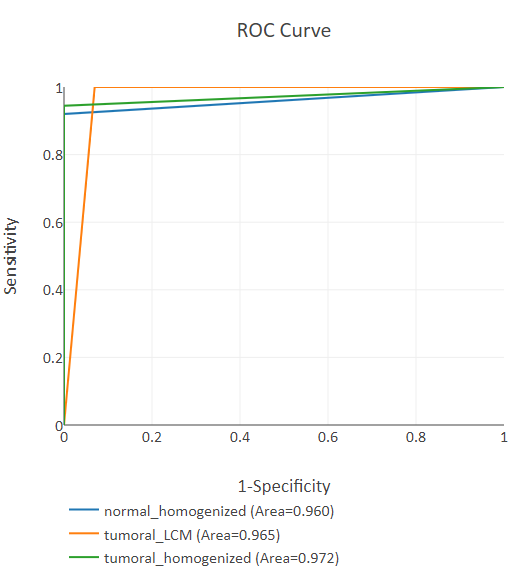
\includegraphics[width=0.4\textwidth]{colorectal_gse21510_ROC.PNG}}
     \subfloat[Curva A]{
       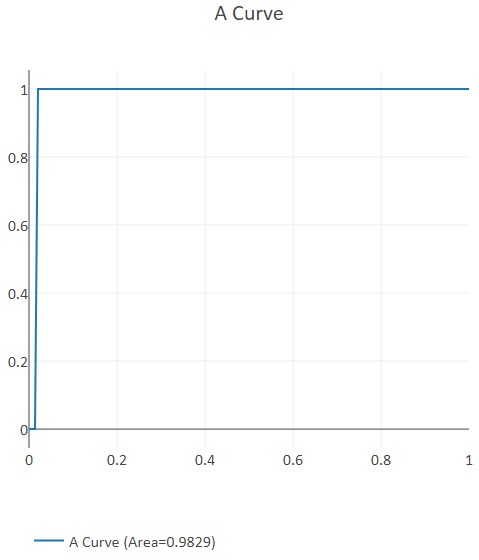
\includegraphics[width=0.4\textwidth]{colorectal_gse21510_A_CURVE.PNG}}
    \caption{Curvas obtenidas para el fichero colorectal\_gse21510.csv.}
    \label{fig:12}
\end{figure}

\bigbreak

El fichero de datos colorectal\_gse21510.csv presenta un total de tres etiquetas para la clase, los nombres de las etiquetas son Normal\_homogenized, Tumoral\_lcm y Tumoral\_homogenized. En esta sección se propone un análisis e interpretación de los resultados obtenidos al aplicar los métodos de evaluación vistos en secciones anteriores. El análisis e interpretación se realiza de forma independiente para las diferentes clases.

\bigbreak

La exactitud presenta una excelente tasa de aciertos, la predicción es correcta para el 98\% de las instancias. La exactitud y el área bajo la curva-A obtienen un resultado similar, la diferencia entre ambos métodos supone un aumento de $0.003$ puntos del área bajo la curva-A sobre la exactitud. La curva ROC muestra una importante capacidad predictiva para las diferentes clases. La curva-A ofrece una representación gráfica que indica una extraordinaria capacidad predictiva.

\bigbreak

La clase Normal\_homogenized presenta una excelente sensibilidad, el 92\% de los registros de esta clase se predicen correctamente. Los métodos de especificidad y precisión obtienen un tasa de aciertos perfecta. La precisión inversa establece que el 98,4\% de los registros no se clasifican de clase Normal\_homogenized cuando la predicción no es Normal\_homogenized. La razón de verosimilitud negativa señala una fuerte reducción en la probabilidad de que los registros no sean de clase Normal\_homogenized cuando la predicción no es Normal\_homogenized. El índice de Youden combina los métodos de sensibilidad y especificidad, el resultado implica que el modelo presenta una elevada capacidad predicativa para la clase Normal\_homogenized. El coeficiente de correlación de Matthews indica un fuerte grado de correlación entre la clase Normal\_homogenized y la predicción (Tabla \ref{tab:3}). La medida-F agrupa los métodos de sensibilidad y precisión, el resultado muestra una gran capacidad predicativa para la clase Normal\_homogenized. El \textit{markedness} indica una excelente capacidad discriminatoria entre la clase Normal\_homogenized y el resto. La media geométrica y la exactitud balanceada muestran una extraordinaria capacidad predicativa. La precisión de optimización presenta un indicador muy elevado para la exactitud en la predicción de la clase Normal\_homogenized. El método de Jaccard establece un fuerte grado de similitud entre la clase Normal\_homogenized y la predicción.

\bigbreak

La clase Tumoral\_lcm presenta un indicador de sensibilidad perfecto, la tasa de acierto es del 100\% para los registros de clase Tumoral\_lcm. La especificidad indica que el 93\% de los registros se predicen de una clase diferente a Tumoral\_lcm cuando la predicción no es de clase Tumoral\_lcm. La precisión establece que la predicción se realiza correctamente para el 97,2\% de los registros que se predicen de clase Tumoral\_lcm. La precisión inversa muestra un indicador perfecto, la clase nunca es Tumoral\_lcm para los registros que no se predicen de clase Tumoral\_lcm. La razón de verosimilitud positiva establece un fuerte aumento en la probabilidad de acierto para los registros que se predicen de clase Tumoral\_lcm. El índice de Youden indica que el modelo presenta una importante capacidad predicativa para la clase Tumoral\_lcm. El coeficiente de correlación de Matthews presenta una fuerte correlación entre la clase Tumoral\_lcm y la predicción. La medida-F establece una excelente capacidad predictiva para los registros en los que la clase o la predicción es Tumoral\_lcm. El \textit{markedness} establece una medida conjunta de precisión y precisión inversa, el resultado representa una tasa alta de acierto para las instancias que se predicen de clase Tumoral\_lcm frente al resto. La media geométrica y la exactitud balanceada presentan una extraordinaria tasa de acierto para los registros de clase Tumoral\_lcm. La precisión de optimización presenta un  indicador elevado de la exactitud del modelo para la clase Tumoral\_lcm. El método de Jaccard establece que una fuerte similitud entre la clase Tumoral\_lcm y la predicción.

\bigbreak

La clase Tumoral\_homogenized presenta una sensibilidad excelente, el 94,4\% de los registros de clase Tumoral\_homogenized se predicen correctamente. La especificidad y la precisión muestran una tasa de aciertos perfecta. La precisión inversa establece que el 99,2\% de los registros no se clasifican de clase Tumoral\_homogenized cuando se predice de una clase diferente. La razón de verosimilitud negativa indica una reducción importante en la probabilidad de que un registro sea de clase Tumoral\_homogenized cuando se predice de una clase diferente. El indice de Youden indica una capacidad discriminatoria notable para la clase Tumoral\_homogenized. El coeficiente de correlación de Matthews establece que existe una fuerte correlación entre la clase Tumoral\_homogenized y la predicción. La medida-F indica una excelente tasa de acierto tanto para instancias que son de clase Tumoral\_homogenized como para instancias que se predicen de clase Tumoral\_homogenized. El \textit{markedness} agrupa los métodos de precisión y precisión inversa, el resultado representa una excelente capacidad discriminatoria entre la clase Tumoral\_homogenized y el resto. La media geometrica y la exactitud balanceada muestran una excelente capacidad predicativa para la clase Tumoral\_homogenized. La precisión de optimización obtiene un indicador muy elevado de la exactitud del modelo para la clase Tumoral\_homogenized. El método de Jaccard presenta un grado de similitud notable entre la clase Tumoral\_homogenized y la predicción.

\clearpage

%%%%%%%%%%%%%%%%%%%%%%%%%%%%%%%%%%%%%%%%%%%%%%%%%%%%%%% RESULTADO

\subsubsection{Fichero breast\_gse42568.csv}

\begin{table}[htp]
    \small
    \centering
    \begin{tabularx}{\columnwidth}{Y Y}
        ACC       & AUAC    \\\hline
        $0.991$   & $0.996$ \\\hline
    \end{tabularx}
    \caption{Resultados globales para el fichero breast\_gse42568.csv.}
    \label{tab:16}
\end{table}

\begin{table}[htp]
    \small
    \centering
    \begin{tabularx}{\columnwidth}{l Y Y}
                &  Normal               & Tumoral       \\\hline
        TPR     &  $0.933$              & $1.000$       \\\hline
        TNR     &  $1.000$              & $0.933$       \\\hline
        PPV     &  $1.000$              & $0.990$       \\\hline
        NPV     &  $0.990$              & $1.000$       \\\hline
        LR+     &  -                    & $15.000$      \\\hline
        LR-     &  $0.067$              & $0.000$       \\\hline
        DOR     &  -                    & -             \\\hline
        YI      &  $0.933$              & $0.933$       \\\hline
        MCC     &  $0.961$              & $0.961$       \\\hline
        DP      &  -                    & -             \\\hline
        $F_{1}$ &  $0.966$              & $0.995$       \\\hline
        MK      &  $0.990$              & $0.990$       \\\hline
        BCR     &  $0.967$              & $0.967$       \\\hline
        GM      &  $0.966$              & $0.966$       \\\hline
        OP      &  $0.957$              & $0.957$       \\\hline
        Jaccard &  $0.933$              & $0.990$       \\\hline
    \end{tabularx}
    \caption{Resultados agrupados por clase para el fichero breast\_gse42568.csv.}
    \label{tab:17}
\end{table}

\bigbreak

\begin{figure}[htp]
    \centering
     \subfloat[Curva ROC]{
       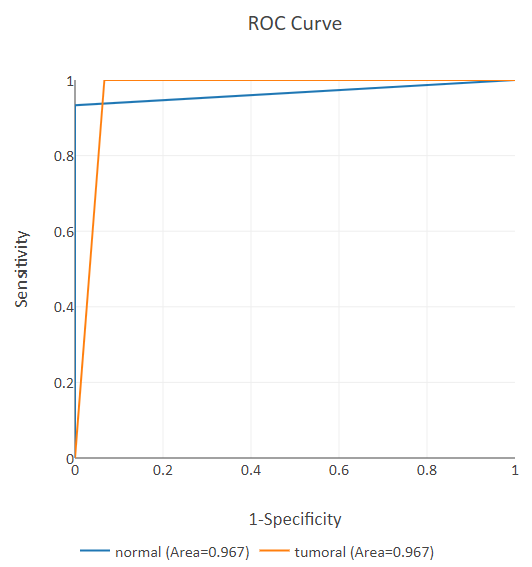
\includegraphics[width=0.4\textwidth]{breast_gse42568_ROC.PNG}}
     \subfloat[Curva A]{
       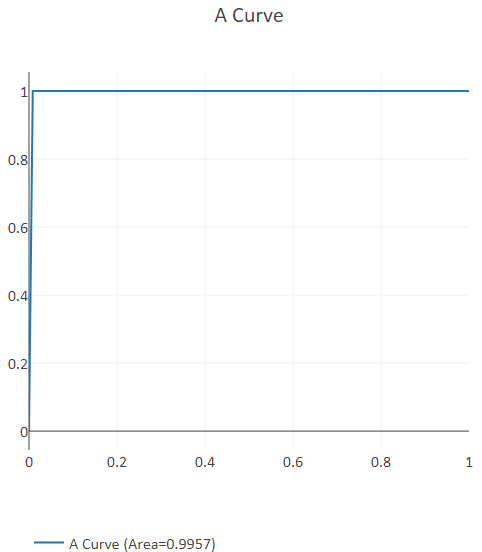
\includegraphics[width=0.4\textwidth]{breast_gse42568_A_CURVE.PNG}}
    \caption{Curvas obtenidas para el fichero breast\_gse42568.csv.}
    \label{fig:13}
\end{figure}

\bigbreak

El fichero de datos breast\_gse42568.csv presenta dos etiquetas para la clase, los nombres de las etiquetas son Tumoral y Normal. En esta sección se propone un análisis e interpretación de los resultados obtenidos al aplicar los métodos de evaluación vistos en secciones anteriores.

\bigbreak

La exactitud presenta un resultado que indica que el modelo tiene una excelente capacidad predictiva, el modelo clasifica correctamente más del 99\% de los registros. El área bajo la curva-A obtiene un valor superior al de la exactitud, el aumento supone una diferencia de 0.005 puntos. La curva ROC ofrece una representación gráfica en la que se muestran las curvas asociadas a la clase Normal y a la clase Tumoral, las dos curvas presentan un comportamiento sobresaliente, en ambos casos las curvas se aproximan al punto de clasificación perfecta. La curva-A muestra una visible capacidad predictiva.

\bigbreak

La clase Normal presenta una sensibilidad excelente por la que 93 de cada 100 registros de clase Normal se predicen correctamente. La especificidad y la precisión muestran un indicador perfecto para la clase Normal, la predicción es correcta para todos los registros que son de clase Tumoral o se predicen de clase Normal. La precisión inversa implica que la predicción es correcta para el 99\% de registros que se predicen de clase Tumoral. El índice de Youden es un método que agrupa los resultados de sensibilidad y especificidad, la capacidad predictiva para ambas clases es notable. El coeficiente de correlación de Matthews muestra una fuerte correlación entre la clase y la predicción. El \textit{markedness} agrupa los métodos de precisión y precisión inversa, en estos términos, el método ofrece un excelente indicador de la capacidad discriminativa del modelo. La exactitud balanceada y la media geométrica son dos indicadores que se obtienen al calcular la media entre la sensibilidad y la especificidad, en ambos casos se establece que el modelo presenta una considerable capacidad predictiva. La precisión de optimización muestra un resultado moderado, en este método se penalizan grandes diferencias entre sensibilidad y especificidad, la diferencia en este caso provoca una reducción de la exactitud en 0,034 unidades.

\bigbreak

La razón de verosimilitud negativa indica una disminución importante de la probabilidad que tienen los registros de ser de clase Normal cuando se predicen de clase Tumoral. La medida-F indica una tasa de acierto excelente para registros en los que la clase o a la predicción tienen asignada la etiqueta Normal. El método de Jaccard establece que existe una gran similitud entre la clase Normal y predicción.

\bigbreak

La clase Tumoral presenta una razón de verosimilitud positiva que señala  un fuerte aumento en la probabilidad de acierto que tiene un registro que se predice de clase Tumoral. El indice de verosimilitud negativo establece nula la probabilidad de clasificar incorrectamente un registro de clase Normal. El método de Jaccard presenta un un indicador que refleja un grado similitud considerable entre la clase Tumoral y la predicción. 

\clearpage


%%%%%%%%%%%%%%%%%%%%%%%%%%%%%%%%%%%%%%%%%%%%%%%%%%%%%%% RESULTADO

\subsubsection{Fichero gastric\_gse79973.csv}

\begin{table}[htp]
    \small
    \centering
    \begin{tabularx}{\columnwidth}{Y Y}
        ACC       & AUAC    \\\hline
        $0.900$   & $0.921$ \\\hline
    \end{tabularx}
    \caption{Resultados globales para el fichero gastric\_gse79973.csv.}
    \label{tab:18}
\end{table}

\begin{table}[htp]
    \small
    \centering
    \begin{tabularx}{\columnwidth}{l Y Y}
                &  Adenocarcinoma       & Normal        \\\hline
        TPR     &  $0.900$              & $0.900$       \\\hline
        TNR     &  $0.900$              & $0.900$       \\\hline
        PPV     &  $0.900$              & $0.900$       \\\hline
        NPV     &  $0.900$              & $0.900$       \\\hline
        LR+     &  $9.000$              & $9.000$       \\\hline
        LR-     &  $0.111$              & $0.111$       \\\hline
        DOR     &  $81.000$             & $81.000$      \\\hline
        YI      &  $0.800$              & $0.800$       \\\hline
        MCC     &  $0.800$              & $0.800$       \\\hline
        DP      &  $1.052$              & $1.052$       \\\hline
        $F_{1}$ &  $0.900$              & $0.900$       \\\hline
        MK      &  $0.800$              & $0.800$       \\\hline
        BCR     &  $0.900$              & $0.900$       \\\hline
        GM      &  $0.900$              & $0.900$       \\\hline
        OP      &  $0.900$              & $0.900$       \\\hline
        Jaccard &  $0.818$              & $0.818$       \\\hline
    \end{tabularx}
    \caption{Resultados agrupados por clase para el fichero gastric\_gse79973.csv.}
    \label{tab:19}
\end{table}

\bigbreak

\begin{figure}[htp]
    \centering
     \subfloat[Curva ROC]{
       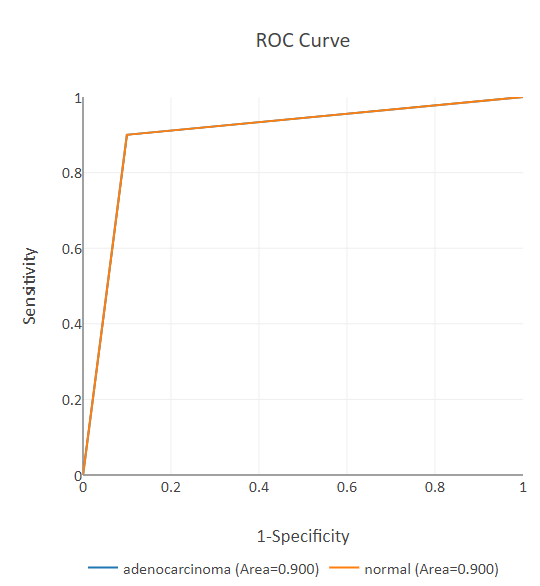
\includegraphics[width=0.4\textwidth]{gastric_gse79973_ROC.PNG}}
     \subfloat[Curva A]{
       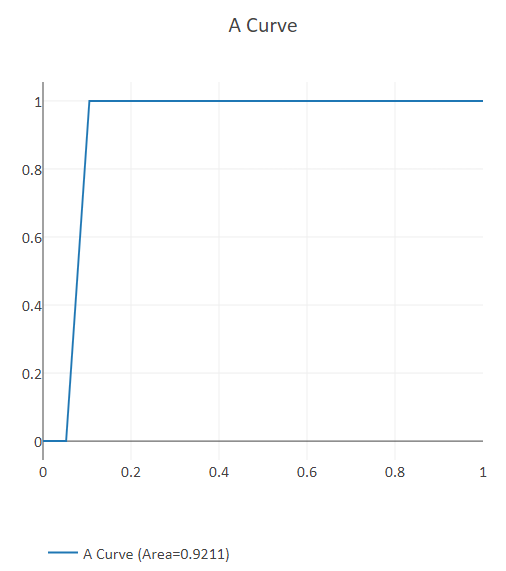
\includegraphics[width=0.4\textwidth]{gastric_gse79973_A_CURVE.PNG}}
    \caption{Curvas obtenidas para el fichero gastric\_gse79973.csv.}
    \label{fig:14}
\end{figure}

\bigbreak

El fichero de datos gastric\_gse79973.csv presenta dos etiquetas para la clase, los nombres de las etiquetas son Adenocarcinoma y Normal. En esta sección se propone un análisis e interpretación de los resultados obtenidos al aplicar los métodos de evaluación vistos en secciones anteriores. Los indicadores que se obtienen son simétricos para ambas clases; así pues, la interpretación se realiza exclusivamente para la clase Adenocarcinoma.

\bigbreak

La exactitud muestra una excelente tasa de aciertos, la predicción es correcta para el 90\% de los registros. La exactitud y el área bajo la curva-A obtienen un resultado similar, la diferencia entre ambos métodos supone un aumento de $0.021$ puntos del área bajo la curva-A sobre la exactitud. La representación gráfica que ofrece la curva ROC indica una tasa de acierto considerable en la predicción de ambas clases. La curva-A ofrece una representación gráfica que muestra una excelente capacidad predictiva.

\bigbreak

Los indicadores de sensibilidad, especificidad, precisión y precisión inversa presentan el mismo resultado, la tasa de acierto en la predicción para estos métodos es del 90\%. El índice de verosimilitud positiva indica un aumento del 40\% en la probabilidad de que la predicción sea correcta para ambas clases (Tabla \ref{tab:2}). El índice de verosimilitud negativa indica una disminución del 45\% en la probabilidad de que la predicción sea incorrecta. El indice de Youden muestra una buena capacidad predictiva a partir de los métodos de sensibilidad y especificidad. El indice de correlación de Matthews establece una fuerte correlación entre clase y predicción (Tabla \ref{tab:3}). El poder discriminante señala una capacidad discriminativa aceptable entre las 2 clases. La medida-F muestra una buena capacidad predictiva, el resultado coincide con los valores de sensibilidad y precisión, ya que el método se define como la media armónica entre ambas métricas. La media geométrica y la exactitud balanceada presentan una tasa de acierto considerable para ambas clases. La precisión de optimización presenta el mismo resultado que la exactitud, el mismo valor de sensibilidad y especificidad provoca que no se produzca ninguna penalización en el indicador. El \textit{markedness} indica una buena tasa de acierto en la predicción de ambas clases. El método de Jaccard presenta un importante grado de similitud entre la clase y la predicción.

\clearpage

%%%%%%%%%%%%%%%%%%%%%%%%%%%%%%%%%%%%%%%%%%%%%%%%%%%%%%% RESULTADO

\subsubsection{Fichero leukemia\_gse14317.csv}

\begin{table}[htp]
    \small
    \centering
    \begin{tabularx}{\columnwidth}{Y Y}
        ACC       & AUAC    \\\hline
        $0.920$   & $0.938$ \\\hline
    \end{tabularx}
    \caption{Resultados globales para el fichero leukemia\_gse14317.csv.}
    \label{tab:20}
\end{table}

\begin{table}[htp]
    \small
    \centering
    \begin{tabularx}{\columnwidth}{l Y Y}
                &  Atl                  & Normal        \\\hline
        TPR     &  $1.000$              & $0.714$       \\\hline
        TNR     &  $0.714$              & $1.000$       \\\hline
        PPV     &  $0.900$              & $1.000$       \\\hline
        NPV     &  $1.000$              & $0.900$       \\\hline
        LR+     &  $3.500$              & -             \\\hline
        LR-     &  $0.000$              & $0.286$       \\\hline
        DOR     &  -                    & -             \\\hline
        YI      &  $0.714$              & $0.714$       \\\hline
        MCC     &  $0.802$              & $0.802$       \\\hline
        DP      &  -                    & -             \\\hline
        $F_{1}$ &  $0.947$              & $0.833$       \\\hline
        MK      &  $0.900$              & $0.900$       \\\hline
        BCR     &  $0.857$              & $0.857$       \\\hline
        GM      &  $0.845$              & $0.845$       \\\hline
        OP      &  $0.753$              & $0.753$       \\\hline
        Jaccard &  $0.900$              & $0.714$       \\\hline
    \end{tabularx}
    \caption{Resultados agrupados por clase para el fichero leukemia\_gse14317.csv.}
    \label{tab:21}
\end{table}

\bigbreak

\begin{figure}[htp]
    \centering
     \subfloat[Curva ROC]{
       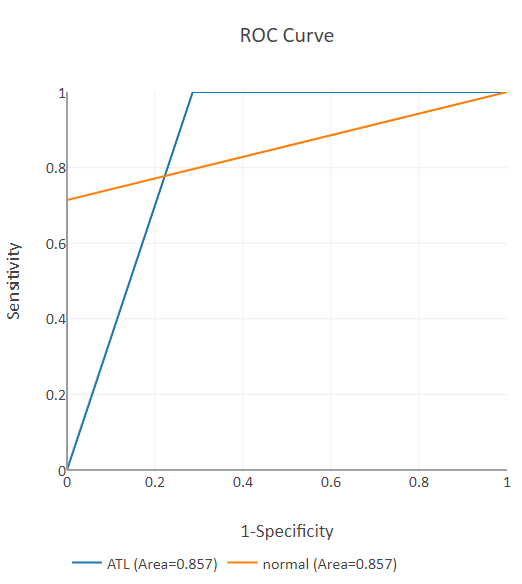
\includegraphics[width=0.4\textwidth]{leukemia_gse14317_ROC.PNG}}
     \subfloat[Curva A]{
       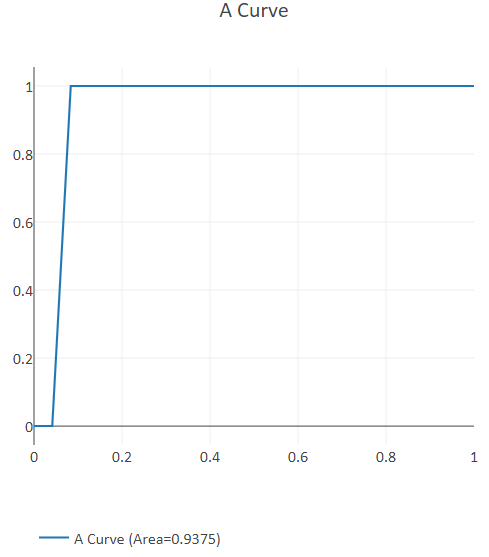
\includegraphics[width=0.4\textwidth]{leukemia_gse14317_A_CURVE.PNG}}
    \caption{Curvas obtenidas para el fichero leukemia\_gse14317.csv.}
    \label{fig:15}
\end{figure}

\bigbreak

El fichero de datos leukemia\_gse14317.csv presenta dos etiquetas para la clase, los nombres de las etiquetas son Atl y Normal. En esta sección se propone un análisis e interpretación de los resultados obtenidos al aplicar los métodos de evaluación vistos en secciones anteriores.

\bigbreak

La exactitud presenta una tasa de aciertos elevada, la predicción es correcta para 92 de cada 100 instancias. La exactitud y el área bajo la curva-A obtienen un resultado similar, la diferencia entre ambos métodos supone un aumento de $0.018$ puntos del área bajo la curva-A sobre la exactitud. La representación gráfica que ofrece la curva ROC muestra una considerable tasa de aciertos en la predicción de ambas clases. La curva-A ofrece una representación gráfica que muestra una excelente capacidad predictiva.

\bigbreak

La clase Atl presenta una sensibilidad perfecta, todos los registros de esta clase se predicen correctamente. La especificidad indica que el 71\% de los registros de clase Normal se predicen de forma correcta. La precisión presenta una tasa de acierto del 90\% para los registros que se predicen de clase Atl. La precisión inversa establece que la predicción es correcta para todos los registros que se predicen de clase Normal. El indice de Youden agrupa los métodos de sensibilidad y especificidad, la tasa de acierto conjunta es notablemente alta. El indice de correlación de Matthews establece una fuerte correlación entre la clase y la predicción (Tabla \ref{tab:3}). El \textit{markedness} combina los métodos de precisión y precisión inversa, el resultado muestra una excelente capacidad discriminativa entre las clases. La media geometrica y la exactitud balanceada son dos métodos que calculan la media entre la sensibilidad y la especificidad, el resultado en ambos casos es elevado. La precisión de optimización muestra una tasa de aciertos considerable, el método penaliza la diferencia de 0,286 puntos entre sensibilidad y especificidad.

\bigbreak

La razón de verosimilitud positiva para la clase Atl presenta un aumento moderado en la probabilidad de que la predicción sea correcta para los registros que se predicen de clase Atl. La medida-F obtiene un excelente indicador de la tasa de acierto para la clase Atl, el método tiene en cuenta tanto a las instancias que son de clase Atl como a las instancias que se predicen de clase Atl. El método de Jaccard señala que existe una gran similitud entre la clase Atl y la predicción.

\bigbreak

La razón de verosimilitud negativa para la clase Normal establece que la probabilidad de que un registro sea de clase Normal disminuye aproximadamente un 30\% cuando el registro se predice de clase Atl (Tabla \ref{tab:2}). La medida-F obtiene un indicador notablemente alto, el método combina la tasa de aciertos para instancias que son de clase Normal y la tasa de aciertos para instancias que se predicen de clase Normal. El método de Jaccard establece un grado similitud importante entre la clase Normal y la predicción.

%Los resultados obtenidos para el fichero leukemia\_gse14317.csv han sido realmente buenos, en general se han obtenido tasas de acierto elevadas. La clase Atl presenta un comportamiento excelente para los registros que son de esta clase o se predicen de esta clase. La clase Normal también presenta buenos resultados

\clearpage

